% Provenance (never printed): see sources/outline_sources.md (Year 3:
% Glen's flow law; mass balance; ice sheets and ice shelves; sea ice;
% permafrost; the cryosphere's contribution to sea level).
% Brief: sources/book5/BRIEFS.md, ch. 24. Curves from figdata/bachelor-3/
% ice_flow.py (Glen slab, the plastic profile against the ETOPO1 Greenland
% transect, the Arkel ice cap) and sea_ice.py (NSIDC March and September
% extents, Stefan's law). Exercise and problem values in the Book 5 scratch
% calculator calc/ch24.py. The Arkel ice cap and the glaciers of the
% exercises are invented.
\chapter{冰川学}\label{ch:b3:glaciology}

沿北纬 \ang{72.5} 自西向东穿越格陵兰岛。冰
面始于距海岸几十千米的内陆，先陡然抬升，随后坡度越来越缓，
抬升至海拔 \qty{3229}{m} 的宽阔峰顶，再下降至东海岸的
山地。将冰面绘成曲线，它近似于一条侧卧的抛物线，
其顶点位于冰盖边缘。本章说明这一形状的来源：
这种形状源于一种材料，受力越大，蠕变越快，
因此它的行为近似于承受不了超过某一应力的载荷。
随后，本章追踪冰从补给它的积雪，到接纳它的海
洋的全过程。
% ledger: data:b5-etopo-greenland

\begin{recall}
冰川、冰盖、冰架、冰山、海冰、永久冻土和冰
期在中学教材中已有介绍。\omterm{def:b3:deformation-mechanisms:flow-law}{流动定律}和\omterm{def:b3:deformation-mechanisms:creep}{位错蠕变}见
第~\ref{ch:b3:deformation-mechanisms}~章；\omterm{def:b3:gravity-geodesy:satgrav}{卫星重力测量}及其测得的
冰盖物质平衡见第~\ref{ch:b3:gravity-geodesy}~章；
冰芯及其氧同位素见第~\ref{ch:b3:stable-isotopes}~章。
海平面收支、冰–反照率反馈和热比容海平面上升，
见本科二年级分册中关于人为
气候变化的一章。潜热和热传导见物理学分册。
\end{recall}

\section{冰作为一种材料}\label{sec:b3:glaciology:material}

冰川冰是一种由相互咬合的冰晶体组成的岩石，
在接近熔点时发生变形。在应力作用下，它通过
晶体内\omterm{def:b3:deformation-mechanisms:dislocation}{位错}的运动发生蠕变，与
第~\ref{ch:b3:deformation-mechanisms}~章中的岩石相同，其\omterm{def:b3:deformation-mechanisms:flow-law}{流动定律}形式也相同：
即应力的幂与阿伦尼乌斯因子之积。

\begin{theorem}[格伦流动定律]\label{thm:b3:glaciology:glen}
在各向同性的冰川冰中，应变速率张量与
偏应力成正比，
\[
\dot\varepsilon_{ij} = A(T)\,\tau_e^{\,n-1}\,\tau'_{ij}, \qquad
\tau_e^2 = \tfrac12\,\tau'_{ij}\tau'_{ij},
\]
取 $n = 3$，\omterm{def:b3:glaciology:glen}{速率因子} $A(T)$ 随温度增大。在
简单剪切中，$\tau_{xz}$ 是唯一非零的偏应力分量，
$\dot\varepsilon_{xz} = A\tau_{xz}^{\,n}$.
\end{theorem}
\index{格伦流动定律}

\begin{proof}
该定律本身是经验性的：它是拟合蠕变实验与
冰川变形资料得到的幂律，其系数与指数一并拟合确定。
在简单剪切中，$\tau'_{xz} = \tau'_{zx} = \tau_{xz}$，其余
分量为零，因此 $\tau_e^2 = \tfrac12(\tau_{xz}^2 +
\tau_{zx}^2) = \tau_{xz}^2$，且 $\dot\varepsilon_{xz} = A\tau_{xz}^{\,n-1}
\tau_{xz}$。
\end{proof}
% ledger: pism:rheology

取 $n = 3$ 时，冰是强非线性流体：应力加倍，
变形速率便增至八倍。其有效黏度 $1/(2A\tau_e^{\,2})$，
并非冰本身的固有性质，而是随应力增大而减小。

\begin{definition}[速率因子（冰）]\label{def:b3:glaciology:glen}
格伦定律中的\emph{速率因子}\index{速率因子（冰）} $A(T)$，又称冰的软度，
写作 $A = A_0\exp(-Q/RT)$，其中 $Q$ 为活化能。
广泛采用的拟合（帕特森与巴德）取 $A_0 =
\qty{3.61e-13}{s^{-1}.Pa^{-3}}$，$Q = \qty{60}{kJ/mol}$，在
\qty{-10}{\celsius} 以下，$A_0 = \qty{1.73e3}{s^{-1}.Pa^{-3}}$，$Q =
\qty{139}{kJ/mol}$，在其以上，更接近熔点，冰
随温度软化得更快。
\end{definition}
% ledger: pism:rheology, codata:R

\begin{center}
\begin{tabular}{lccc}
\hline
温度 & \qty{-25}{\celsius} & \qty{-10}{\celsius} & \qty{0}{\celsius}\\
$A$（\unit{Pa^{-3}.\text{年}^{-1}}） & \num{2.7e-18} & \num{1.4e-17} & \num{1.4e-16}\\
\hline
\end{tabular}
\end{center}

冰在熔点时的流动速度约为
\qty{-25}{\celsius} 时相同应力下的五十倍。冰川中的应力量级
约为一巴，即 \qty{e5}{Pa}。
% ledger: pism:rheology

冰川以两种方式运动：其冰体处处通过蠕变变形；
在床面处于熔点之处，冰川还可能滑动。

\begin{definition}[底部滑动]\label{def:b3:glaciology:sliding}
\emph{底部滑动}\index{底部滑动}是指冰川沿
床面之上的运动，发生在一层薄水膜或软湿沉积物上。它
要求床面处于熔点；冰川若冻结于床面，则只能
靠冰体蠕变运动。
\end{definition}
% ledger: nsidc:glacier-flow

\section{冰川流动}\label{sec:b3:glaciology:flow}

\begin{theorem}[平行边板状冰体的流动]\label{thm:b3:glaciology:slab}
厚度为 $H$、密度为 $\rho$ 的板状冰体覆于坡度为
$\alpha$ 的床面上，以简单剪切方式沿坡流动，床面滑动速度为 $u_b$。在
离床面高度 $z$ 处，剪应力为 $\tau = \rho g(H - z)\sin\alpha$，
速度为
\[
u(z) = u_b + \frac{2A}{n + 1}(\rho g\sin\alpha)^n\left[H^{n+1} - (H -
z)^{n+1}\right],
\]
单位宽度的通量为 $q = u_bH + \dfrac{2A}{n + 2}(\rho
g\sin\alpha)^nH^{n+2}$。床面剪应力为 $\tau_b = \rho gH\sin\alpha$。
\end{theorem}

\begin{proof}
离高度 $z$ 以上的冰体，单位面积重量为 $\rho g(H - z)$，其
沿坡分量 $\rho g(H - z)\sin\alpha$，由其底面的
剪应力平衡，冰面不受应力。
由格伦定律，$\mathrm du/\mathrm dz = 2\dot\varepsilon_{xz} = 2A\tau^n$，
从床面（此处 $u = u_b$）积分，得 $u(z)$；再对 $u$ 从 0 到 $H$
积分，得 $q$。
\end{proof}

板片上部速度变化很小，靠近床面处则变化很快，
那里应力最大：当 $n = 3$ 时，剪切集中在
最底层。表面速度随 $H^{n+1} = H^4$ 增大，
并与坡度的三次方成正比：厚度为两倍的冰川，流速快十六倍。

\begin{definition}[浅冰近似]\label{def:b3:glaciology:sia}
\emph{浅冰近似}\index{浅冰近似}将
厚度相对宽度很小的冰盖，局部视为
两侧平行的板片：每一处的冰体在
\emph{驱动应力} $\tau_d = \rho gH|\nabla s|$ 作用下以简单剪切方式变形，$s$ 为
地表高程，通量按板片公式计算，采用局部
厚度与地表坡度。
\end{definition}

在\omterm{def:b3:glaciology:sia}{浅冰近似}中，床面应力由
冰体的形状决定。由于应变率与应力的三次方成正比，应力的微小
增加会使流动大幅增加，进而使冰体变薄，
应力随之再次下降，应力始终保持在狭窄范围内，
无论冰体规模大小。将此推向极限，设想一种材料，
在屈服应力 $\tau_0$ 以下完全不变形，超过该值后则无限制地变形，
其形状便可由此得出。

\begin{proposition}[理想塑性冰盖剖面]\label{prop:b3:glaciology:nye}
屈服应力为 $\tau_0$ 的理想塑性冰盖，位于水平平坦的
床面上，距其边缘 $x$ 处，地表高度为
\[
h(x) = \sqrt{\frac{2\tau_0x}{\rho g}} .
\]
\end{proposition}
\index{理想塑性冰盖剖面}

\begin{proof}
处处床面应力等于屈服应力：$\rho gh\,\mathrm
dh/\mathrm dx = \tau_0$，坡度很小。于是 $\mathrm d(h^2)/\mathrm
dx = 2\tau_0/(\rho g)$，且在边缘处 $h = 0$。
\end{proof}

\begin{omfigure}
\begin{tikzpicture}
\begin{groupplot}[group style={group size=2 by 1, horizontal sep=1.5cm},
  height=0.4\linewidth,
  tick label style={font=\scriptsize}, label style={font=\small}, title style={font=\small}]
\nextgroupplot[width=0.38\linewidth, xlabel={$u/u_s$}, ylabel={离床面高度，$z/H$},
  xmin=0, xmax=1.05, ymin=0, ymax=1, title={板片},
  legend style={font=\scriptsize, at={(0.03,0.97)}, anchor=north west}]
% computed in figdata/bachelor-3/ice_flow.py
\addplot[omThm, thick] table[x=u3, y=zeta] {figdata/out/bachelor-3-ice_flow-slab.dat};
\addlegendentry{$n = 3$}
\addplot[omDef, thick, densely dashed] table[x=u1, y=zeta] {figdata/out/bachelor-3-ice_flow-slab.dat};
\addlegendentry{$n = 1$}
\addplot[omMeth, thick] table[x=u3b, y=zeta] {figdata/out/bachelor-3-ice_flow-slab.dat};
\addlegendentry{$n = 3$，滑动}
\nextgroupplot[width=0.58\linewidth, xlabel={沿北纬 \ang{72.5}、距西经 \ang{58} 的距离（\unit{km}）},
  ylabel={海拔（\unit{m}）}, xmin=0, xmax=1270, ymin=-500, ymax=3700,
  title={格陵兰}, scaled x ticks=false, xticklabel style={/pgf/number format/1000 sep={}},
  scaled y ticks=false, yticklabel style={/pgf/number format/1000 sep={}},
  legend style={font=\scriptsize, at={(0.5,0.03)}, anchor=south}]
\addplot[black, thin] table[x=x, y=h] {figdata/out/bachelor-3-ice_flow-gl.dat};
\addlegendentry{冰面与陆地表面}
\addplot[omThm, thick, densely dashed] table[x=x, y=h] {figdata/out/bachelor-3-ice_flow-nye-w.dat};
\addlegendentry{塑性剖面}
\addplot[omThm, thick, densely dashed, forget plot] table[x=x, y=h] {figdata/out/bachelor-3-ice_flow-nye-e.dat};
\draw[black!40] (axis cs:0,0) -- (axis cs:1270,0);
\node[font=\scriptsize, omThm, align=center] at (axis cs:330,2900) {$\tau_0 = $\\ \qty{72}{kPa}};
\node[font=\scriptsize, omThm, align=center] at (axis cs:1040,2900) {$\tau_0 = $\\ \qty{108}{kPa}};
\end{groupplot}
\end{tikzpicture}

\par\smallskip{\small 左图为板片状冰体沿厚度方向的速度分布，以
地表速度归一化：格伦定律（$n = 3$）使剪切集中在床面附近，线性
流体（$n = 1$）则使其分散；存在滑动时，整个剖面
平移。右图为沿北纬 \ang{72.5} 的格陵兰地表（ETOPO1 Ice
Surface, NOAA NCEI），以及拟合其两侧的塑性剖面，
拟合范围为高于 \qty{1000}{m} 的部分，床面取海平面。拟合
得到的屈服应力为 \qty{72}{kPa} 和 \qty{108}{kPa}，约为一巴，与
真实冰川的数量级相当；拟合未能反映陡峭边缘处的情况，那里床面与融化
作用至关重要。}\label{fig:b3:glaciology:flow}
\end{omfigure}
% ledger: data:b5-etopo-greenland, pism:rheology

\section{物质平衡}\label{sec:b3:glaciology:mass-balance}

冰川由降雪补给，并通过融化、蒸发，以及在
到达水体时断裂脱落而失去冰量。
% ledger: nsidc:glacier-zones

\begin{definition}[物质平衡；积累区与消融区；平衡线]\label{def:b3:glaciology:mass-balance}
\emph{冰川物质平衡}\index{冰川物质平衡}是指冰川
质量在一年内的变化，通常以水当量（米）表示，
并按其面积取平均。\emph{表面物质
平衡}\index{表面物质平衡}是由表面过程引起的部分，
即降雪减去融化、径流和升华；其余部分则
通过\omterm{def:b3:glaciology:grounding-line}{崩解}，以及在底部或浮冰下的融化而失去。
\emph{积累区}\index{积累区}是指
表面物质平衡在一年内为正的那部分表面，
\emph{消融区}\index{消融区}是指其为负的那部分，
而\emph{平衡线高度}\index{平衡线高度}
（ELA）则是二者之间分界线的海拔，该处物质平衡为零。
\end{definition}

\begin{omfigure}
\centering
\begin{tikzpicture}[>=stealth, font=\small, x=1cm, y=1cm]
% bed and surface of a valley glacier, long section
\fill[black!12] (0,0) -- (0,4.6) .. controls (2,3.6) and (6,1.4) .. (11,0) -- cycle;
\fill[omSea!45] (0,4.6) .. controls (2,3.6) and (6,1.4) .. (11,0)
  -- (11,0) .. controls (8,1.0) and (4,3.2) .. (0.6,5.4) -- (0,5.6) -- cycle;
\draw[thick, black!70] (0,4.6) .. controls (2,3.6) and (6,1.4) .. (11,0);
\draw[thick, omDef] (0,5.6) -- (0.6,5.4) .. controls (4,3.2) and (8,1.0) .. (11,0);
% equilibrium line
\draw[omThm, densely dashed, thick] (5.0,2.76) -- (5.0,4.6);
\node[omThm, font=\scriptsize, anchor=south] at (5.0,4.6) {平衡线（ELA）};
% balance arrows
\foreach \x/\y in {1.2/5.02, 2.4/4.27, 3.6/3.56} {\draw[->, omDef, thick] (\x,\y+0.55) -- (\x,\y+0.05);}
\foreach \x/\y in {6.4/2.02, 7.6/1.42, 8.8/0.86} {\draw[->, omThm, thick] (\x,\y+0.02) -- (\x,\y+0.52);}
\node[omDef, font=\scriptsize, align=center] at (2.4,6.2) {积累区：\\获得积雪};
\node[omThm, font=\scriptsize, align=center] at (8.6,2.5) {消融区：\\失去冰量};
% flow lines, computed inside the ice: buried in the accumulation zone, emerging in the ablation zone
\draw[->, black!60] plot[smooth] coordinates {(1.00,5.14) (1.98,4.28) (2.95,3.54) (3.93,2.93) (4.90,2.43) (5.88,2.00) (6.85,1.62) (7.83,1.24) (8.80,0.86)};
\draw[->, black!60] plot[smooth] coordinates {(2.20,4.39) (2.84,3.89) (3.48,3.43) (4.11,3.02) (4.75,2.67) (5.39,2.36) (6.03,2.08) (6.66,1.82) (7.30,1.56)};
\draw[->, black!60] plot[smooth] coordinates {(3.40,3.67) (3.74,3.44) (4.08,3.21) (4.41,3.00) (4.75,2.81) (5.09,2.63) (5.42,2.47) (5.76,2.32) (6.10,2.17)};
\node[font=\scriptsize, anchor=north east] at (10.9,-0.1) {冰舌};
\node[font=\scriptsize] at (3.0,1.4) {基岩};
\end{tikzpicture}

\par\smallskip{\small 处于平衡状态的山谷冰川
纵剖面示意图。平衡线以上，每年的积雪被掩埋并
带入冰川内部；平衡线以下，表面每年失去冰量，
由深处上升的冰补充。流线（灰色）在
\omterm{def:b3:glaciology:mass-balance}{积累区}向下倾斜，在\omterm{def:b3:glaciology:mass-balance}{消融区}向上升起；流动把
一处的盈余输送到另一处的亏损。}\label{fig:b3:glaciology:zones}
\end{omfigure}
% ledger: nsidc:glacier-zones, nsidc:glacier-flow

在冰盖和高山冰川上，雪并不会在一个季节内
变成冰。它会被后来的雪掩埋、压实并重结晶。

\begin{definition}[粒雪；气孔封闭]\label{def:b3:glaciology:firn}
\emph{粒雪}\index{粒雪}是至少经历过一个融化季节的雪，
正被压实成冰：密度大于雪，仍可透气。
\emph{气孔封闭}\index{气孔封闭}是粒雪压实过程中的一个节点，
此时密度约为 \qtyrange{820}{830}{kg/m^3}，
颗粒间的孔隙被封闭成气泡，其中的空气与
大气隔绝。
\end{definition}

在极地冰盖上，\omterm{def:b3:glaciology:firn}{气孔封闭}位于地表以下 \qtyrange{50}{120}{m} 处，
取决于温度、积累量和杂质含量；
因此冰芯气泡中的空气比周围的冰更年轻，
正如第~\ref{ch:b3:stable-isotopes}~章所回顾的。对于大多数冰川，
由雪变成冰的过程需要一百多年。
% ledger: nsidc:firn, firn:close-off

冰川不会立即对气候变化作出响应。其厚度
须先发生变化，其长度才能随之改变。

\begin{proposition}[冰川响应时间]\label{prop:b3:glaciology:response}
设典型厚度为 $H$、末端物质平衡为 $b_t <
0$（单位为每年冰的米数）的冰川，对气候变化的响应时间
约为以下量级：
\[
\tau = \frac{H}{-b_t} .
\]
\end{proposition}

\begin{proof}
若整个冰川的物质平衡变化 $\delta b$，则其体积随之改变，
直至末端处的面积损失或增加（此处物质平衡为 $b_t$）将其抵消：
即每单位宽度满足 $L\,\delta b = -b_t\,\delta L$，其中 $L$ 为冰川长度。
所需的体积变化约为 $H\,\delta L$，而
驱动其变化的初始失衡为每年 $L\,\delta b$，故
所需时间为 $H\,\delta L/(L\,\delta b) = H/(-b_t)$ 年。
\end{proof}

一条厚 \qty{200}{m}、冰舌处每年失去 \qty{5}{m} 冰量的冰川，
约需四十年才能作出响应。因此，冰川滞后于气候变化：
现今的冰川即使在
气温停止上升之后，仍将在数十年内继续失去质量。
% ledger: ar6ch9:glaciers

\section{冰盖与冰架}\label{sec:b3:glaciology:ice-sheets}

格陵兰与南极的冰盖储存了超过
\qty{99}{\percent} 的陆地冰。格陵兰冰盖面积为 \qty{1.7}{\mega
km^2}，最厚处超过 \qty{3}{km}；南极冰盖面积
约 \qty{14}{\mega km^2}，最厚处接近 \qty{4.9}{km}。南极冰盖的许多
部分坐落在海平面以下的冰床上。
% ledger: nsidc:ice-sheets, ar6ch9:faq91

\begin{definition}[冰流]\label{def:b3:glaciology:ice-stream}
\emph{冰流}\index{冰流}是冰盖中一条以
远快于两侧冰体的速度流动的带状区域，主要依靠滑动或
软湿床层的变形，将冰盖内部的大部分冰
输送至其边缘。
\end{definition}

\begin{definition}[接地线；崩解]\label{def:b3:glaciology:grounding-line}
\emph{接地线}\index{接地线}是支撑于床面上的冰
开始漂浮的界线：界线以海侧的冰为
冰架或漂浮冰舌。\emph{崩解}\index{崩解}是指冰块
（即冰山）从冰川或冰架的前缘断裂脱落的过程，该前缘
终止于水体。
\end{definition}

冰架浮于水面，因此其融化不会抬高海平面。但冰架
两侧及其搁浅的海底隆起处受到约束，此处的阻力
抵抗后方冰体的流动，故它们起到
\emph{支撑}作用。2002 年拉森~B 冰架\omterm{def:b3:glaciology:grounding-line}{崩解}后，
此前向其供冰的冰川加速，最多达八倍。
% ledger: nsidc:ice-shelves

\begin{proposition}[漂浮条件]\label{prop:b3:glaciology:flotation}
密度为 $\rho_i$、厚度为 $H$ 的冰位于海平面以下深度
为 $D$ 的床面上，处于密度为 $\rho_w$ 的海水中。若 $H < (\rho_w/\rho_i)D$，则冰漂浮。
取 $\rho_i = \qty{917}{kg/m^3}$，$\rho_w = \qty{1025}{kg/m^3}$，则
\omterm{def:b3:glaciology:grounding-line}{接地线}位于冰厚为 $1.12\,D$ 处。
\end{proposition}

\begin{proof}
漂浮的冰排开与其自身重量相等的水：厚度为 $H$ 的冰柱
需要的吃水深度为 $\rho_iH/\rho_w$。若水深大于该吃水深度，
则冰漂浮。
\end{proof}
% ledger: iapws:ice-density, noaa:seawater-1025

\begin{omfigure}
\centering
\begin{tikzpicture}[>=stealth, font=\small, x=1cm, y=1cm]
% sea and bed
\fill[omSea!50] (4.2,0) rectangle (11,-2.8);
\fill[black!15] (0,-0.9) -- (2.2,-2.0) -- (4.6,-1.6) -- (7.0,-2.3) -- (11,-2.6)
  -- (11,-3.2) -- (0,-3.2) -- cycle;
\draw[thick, black!60] (0,-0.9) -- (2.2,-2.0) -- (4.6,-1.6) -- (7.0,-2.3) -- (11,-2.6);
% grounded ice and ice shelf
\fill[white] (0,-0.9) -- (0,2.4) .. controls (2,2.2) and (3.6,1.4) .. (4.6,0.2)
  -- (9.2,0.12) -- (9.2,-1.0) -- (4.6,-1.6) -- (2.2,-2.0) -- cycle;
\draw[thick, omDef] (0,2.4) .. controls (2,2.2) and (3.6,1.4) .. (4.6,0.2) -- (9.2,0.12)
  -- (9.2,-1.0) -- (4.6,-1.6);
\draw[thick] (0,0) -- (0,0);
\draw[omDef!60, thin] (0,0) -- (4.3,0); \draw[omDef!60, thin] (9.2,0) -- (11,0);
\node[font=\scriptsize, anchor=south west] at (0.05,0.02) {海平面};
% icebergs
\fill[white] (10.1,0.1) rectangle (10.6,-0.7); \draw[omDef] (10.1,0.1) rectangle (10.6,-0.7);
% labels
\fill[omThm] (4.6,-1.6) circle (0.07);
\draw[omThm, ->] (4.0,-2.6) node[anchor=north, font=\scriptsize] {接地线} -- (4.55,-1.68);
\node[font=\scriptsize] at (1.4,1.1) {接地冰盖};
\node[font=\scriptsize] at (6.9,-0.7) {漂浮冰架};
\node[font=\scriptsize, anchor=south] at (9.2,0.2) {崩解前缘};
\node[font=\scriptsize, anchor=north, align=center] at (10.35,-0.8) {冰山};
\node[font=\scriptsize, align=center] at (2.1,-2.55) {床面向内陆 \\加深};
\draw[->, black!60, thick] (2.2,1.6) -- (3.6,1.0);
\draw[->, black!60, thick] (5.4,-0.2) -- (7.0,-0.2);
\node[font=\scriptsize, align=center, omMeth] at (7.0,1.2) {支撑作用：冰架两侧与 \\接地隆起处的阻力};
\draw[->, omMeth, thick] (7.6,0.6) -- (6.6,0.6);
\end{tikzpicture}

\par\smallskip{\small 海洋冰盖的示意剖面，
未按比例绘制。冰层位于海平面以下的床面上，床面向陆内加深；在\omterm{def:b3:glaciology:grounding-line}{接地线}处，
冰开始浮起成为冰架，冰架通过前缘\omterm{def:b3:glaciology:grounding-line}{崩解}和底部融化而失去冰量。
冰架的阻力来自其两侧受约束之处，
以及海底隆起处，二者共同阻碍了
接地冰的流动。}\label{fig:b3:glaciology:grounding}
\end{omfigure}
% ledger: nsidc:ice-shelves, ar6ch9:misi

床面向陆内加深时，\omterm{def:b3:glaciology:grounding-line}{接地线}是脆弱的。在
水较深之处，\omterm{def:b3:glaciology:grounding-line}{接地线}处的冰较厚，由浮力条件可知，
并由板片定理，较厚冰柱的通量
随其厚度急剧增长。若\omterm{def:b3:glaciology:grounding-line}{接地线}沿这样的斜坡后退，
则会到达更厚的冰，它排泄更多冰量、变薄更快，
并使\omterm{def:b3:glaciology:grounding-line}{接地线}进一步后退。

\begin{definition}[海洋冰盖不稳定性]\label{def:b3:glaciology:misi}
\emph{海洋冰盖不稳定性}\index{海洋冰盖不稳定性}
（MISI）是指被提出的一种自增强后退：冰盖的\omterm{def:b3:glaciology:grounding-line}{接地线}
位于向陆内下倾的床面上，若无冰架的支撑，
\omterm{def:b3:glaciology:grounding-line}{接地线}在这种床面上本质上是不稳定的，
直至到达向上倾斜的床面为止。
\end{definition}

冰架即使在下倾斜坡上，也能使\omterm{def:b3:glaciology:grounding-line}{接地线}保持原位。
若模拟中移除全部南极冰架且不允许其重新形成，
经此不稳定性，在 500
年内损失的冰量相当于 \qtyrange{2}{10}{m} 海平面，其中 \qtyrange{2}{5}{m} 来自西
南极。位于海平面以上、主要坐落于基岩上的冰盖，如
格陵兰冰盖，其主要的自增强过程则不同：表面融化并降低后，
所处空气更暖，融化更多。
% ledger: ar6ch9:misi, ar6ch9:faq91

\begin{definition}[海平面当量]\label{def:b3:glaciology:sle}
陆地冰体质量的\emph{海平面当量}\index{海平面当量}是指
若将其融化后的水均匀铺布于现今海洋之上，
所引起的全球平均海平面上升幅度。
\end{definition}

\begin{proposition}[冰体质量的海平面当量]\label{prop:b3:glaciology:sle}
设位于海平面以上的冰体质量为 $M$，将其铺布于面积为 $A_o$ 的海洋上，
并化为密度为 $\rho_w$ 的水，则海平面上升 $M/(\rho_wA_o)$，
即每 \qty{360}{Gt} 约使海平面上升 \qty{1}{mm}。
\end{proposition}

\begin{proof}
水的体积为 $M/\rho_w$，分布于面积 $A_o$ 上。取
冰盖物质平衡评估中采用的每毫米 \qty{360}{Gt} 换算关系，
$A_o\rho_w = \qty{3.6e17}{kg/m}$，相当于面积约为
\qty{3.6e8}{km^2} 的海洋，其中水的密度取淡水值。
\end{proof}
% ledger: data:b5-imbie

已位于海平面以下的冰会排开海水，因此计入较少：
南极 \qty{30}{\mega km^3} 的冰相当于约
\qty{58}{m} 的海平面上升，小于其质量
除以 \qty{360}{Gt/mm} 所得的值。
% ledger: nsidc:ice-sheets

\begin{omfigure}
\centering
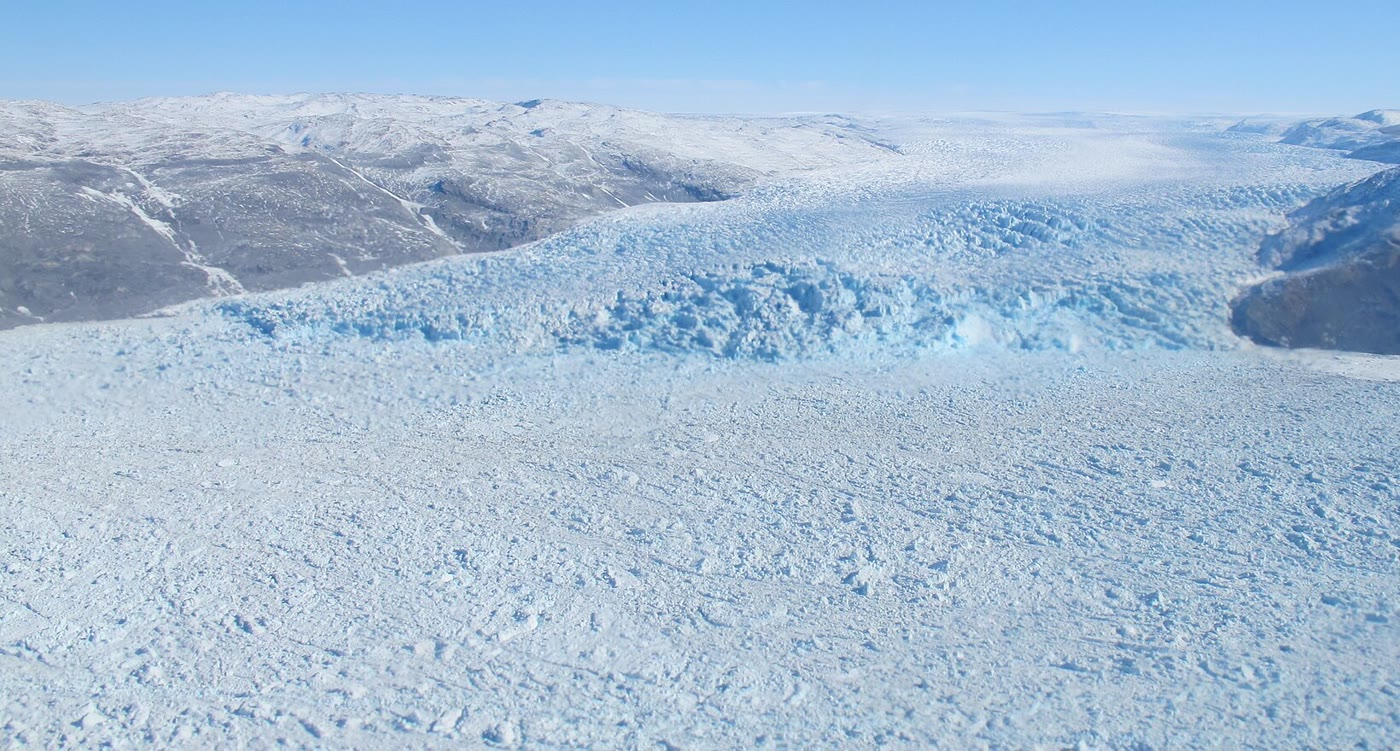
\includegraphics[width=0.82\linewidth]{images/book5/b3-greenland-outlet.jpg}

\par\smallskip{\small 格陵兰冰盖的一条出口冰川，
夹于山脉之间，在\omterm{def:b3:glaciology:grounding-line}{崩解}前缘处入海，画面中部为断裂的
蓝色冰壁；前方峡湾被
崩落冰块与海冰堵塞。由 NASA 的
Operation IceBridge 项目飞机于 2014 年 4 月拍摄（NASA / Jim Yungel，
公有领域）。}\label{fig:b3:glaciology:outlet}
\end{omfigure}
% ledger: photo:b3-greenland-outlet

\begin{inthefield}[冰盖上的营地]
\begin{minipage}[t]{0.55\linewidth}\vspace{0pt}
在冰盖上，冰川学家的仪器靠雪橇运送，人员住在
帐篷中。为测量冰的移动速度，他们把一根标杆冻入
雪中，并在其上安装卫星导航接收机的天线。
大地测量学所用的接收机可将位置精确到几厘米以内，因此
相隔数周或数个季节重复测得的位置，可得冰的速度与
方向；再次测量标杆的高度，则可得其下冰层的
变薄或增厚。
\end{minipage}\hfill
\begin{minipage}[t]{0.42\linewidth}\vspace{0pt}
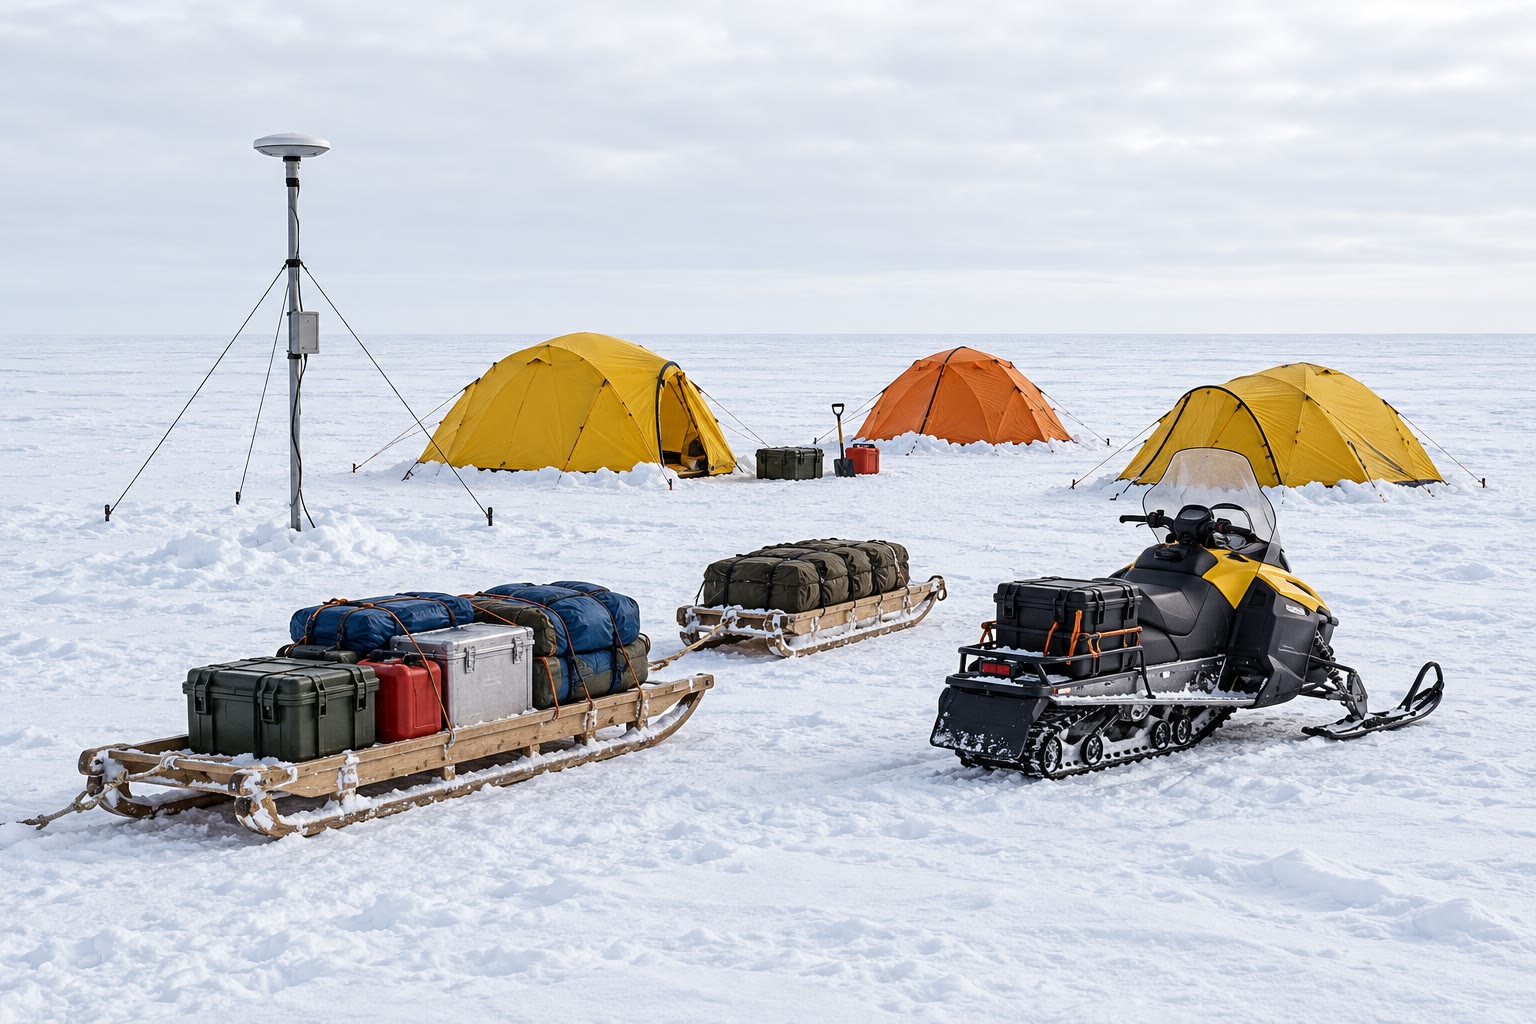
\includegraphics[width=\linewidth]{images/book5/ai/b3-glaciology-camp.jpg}

{\scriptsize 冰盖上的野外营地：帐篷、雪橇和一
辆雪地摩托，以及桅杆上由拉索固定的卫星导航天线
（AI 生成插图）。}
\end{minipage}
\end{inthefield}
% ledger: gps:high-end

\section{海冰与永久冻土}\label{sec:b3:glaciology:sea-ice}

海冰在海洋中形成、增长和融化。在北极，海冰面积
3 月达到最大，9 月达到最小。
% ledger: nsidc:sea-ice-def

\begin{definition}[海冰范围]\label{def:b3:glaciology:sea-ice}
\emph{海冰范围}\index{海冰范围}是指卫星地图中
海冰覆盖超过 \qty{15}{\percent} 表面的各网格单元的总面积。
其值大于海冰面积，
后者只计冰体本身。
\end{definition}
% ledger: nsidc:sea-ice-def

自 1979 年卫星开始测绘以来，北极\omterm{def:b3:glaciology:sea-ice}{海冰范围}已缩小，
3 月缩小较少，9 月缩小更多：9 月每十年减少 \qty{0.74}{\mega km^2}，
约相当于 1981--2010 年均值的 \qty{12}{\percent}（每十年），与之相比，
3 月为 \qty{0.38}{\mega km^2}，即 \qty{2.5}{\percent}。
迄今最小的 9 月范围为 \qty{3.57}{\mega km^2}，出现于 2012 年。北极海冰
反射 \qtyrange{50}{70}{\percent} 的阳光，开阔洋面
仅反射约 \qty{6}{\percent}：海冰消失使表面变暗，
即本科二年级分册中的冰–反照率反馈。
% ledger: data:b5-nsidc-extent, nsidc:sea-ice-reflect

海冰在底部生长，海水在其上凝固，凝固所释放的潜热
必须通过冰层向上传导至寒冷的空气中。

\begin{theorem}[斯特藩定律]\label{thm:b3:glaciology:stefan}
设海冰的热导率为 $k_i$，密度为 $\rho_i$，熔化潜热为
$L$，其表面温度比其下方海水的凝固点低 $\Delta T$，
若来自海洋的热量
可忽略，则海冰厚度按下式增长：
\[
h(t)^2 - h(0)^2 = \frac{2k_i\,\Delta T}{\rho_iL}\,t .
\]
在厚度为 $h_s$、热导率为 $k_s$ 的雪层覆盖之下，
增长速率为 $\mathrm dh/\mathrm dt = \Delta T/[\rho_iL(h/k_i + h_s/k_s)]$。
\end{theorem}

\begin{proof}
薄冰中的温度呈线性分布，从底部的凝固点
变化到顶部的表面温度，因此通过冰层的热流量为
$k_i\Delta T/h$；若冰与雪串联，则为 $\Delta T/(h/k_i +
h_s/k_s)$。凝固一层厚度为 $\mathrm dh$ 时，释放 $\rho_iL\,\mathrm dh$
单位面积的热量，这些热量须由该热流量带走：$\rho_iL\,\mathrm dh/\mathrm dt
= k_i\Delta T/h$。于是 $\mathrm d(h^2)/\mathrm dt = 2k_i\Delta T/(\rho_iL)$。
\end{proof}

取 $k_i = \qty{2.03}{W.m^{-1}.K^{-1}}$，$L = \qty{3.34e5}{J/kg}$，
$\rho_i = \qty{917}{kg/m^3}$，表面比凝固点低 \qty{20}{K} 时，
冰层在一百天内增长 \qty{1.5}{m}，在两百天内增长 \qty{2.1}{m}。
雪的热导率为 \qty{0.30}{W.m^{-1}.K^{-1}}，是良好的绝缘体：
\qty{20}{cm} 厚的雪层可使增长速率减半以上。厚冰增长缓慢，
薄冰增长迅速：该定律使冰层厚度
在经夏季熔化之后趋于均匀。
% ledger: cice:constants, iapws:ice-density

\begin{omfigure}
\begin{tikzpicture}
\begin{groupplot}[group style={group size=2 by 1, horizontal sep=1.5cm},
  width=0.48\linewidth, height=0.4\linewidth,
  tick label style={font=\scriptsize}, label style={font=\small}, title style={font=\small}]
\nextgroupplot[xlabel={年份}, ylabel={范围 (\unit{\mega km^2})}, xmin=1977, xmax=2028,
  ymin=0, ymax=18, title={北极海冰范围},
  xticklabel style={/pgf/number format/1000 sep={}},
  legend style={font=\scriptsize, at={(0.03,0.66)}, anchor=west}]
% computed in figdata/bachelor-3/sea_ice.py
\addplot[omDef, thick, mark=*, mark size=0.9pt] table[x=year, y=mar] {figdata/out/bachelor-3-sea_ice-extent.dat};
\addlegendentry{3 月}
\addplot[omThm, thick, mark=*, mark size=0.9pt] table[x=year, y=sep] {figdata/out/bachelor-3-sea_ice-extent.dat};
\addlegendentry{9 月}
\addplot[black!60, densely dashed, forget plot] table[x=year, y=mar] {figdata/out/bachelor-3-sea_ice-trend.dat};
\addplot[black!60, densely dashed, forget plot] table[x=year, y=sep] {figdata/out/bachelor-3-sea_ice-trend.dat};
\nextgroupplot[xlabel={凝固天数}, ylabel={冰厚 (\unit{m})}, xmin=0, xmax=200,
  ymin=0, ymax=2.4, title={增长，$\Delta T = \qty{20}{K}$},
  legend style={font=\scriptsize, at={(0.97,0.03)}, anchor=south east}]
\addplot[omMeth, thick] table[x=day, y=h0] {figdata/out/bachelor-3-sea_ice-stefan.dat};
\addlegendentry{裸冰}
\addplot[omDef, thick, densely dashed] table[x=day, y=hs] {figdata/out/bachelor-3-sea_ice-stefan.dat};
\addlegendentry{\qty{20}{cm} 雪层之下}
\end{groupplot}
\end{tikzpicture}

\par\smallskip{\small 左图，北极海冰的平均范围，3 月与
9 月，时段为 1979--2026 年（NSIDC Sea Ice Index，第~4~版），附最小二乘
趋势线（虚线）：每十年分别为 \qty{-0.38}{\mega km^2} 和 \qty{-0.74}{\mega km^2}。右图，
海冰因传导而增长的情况，表面比凝固点低
\qty{20}{K}，不计海洋热量：裸冰按斯特藩定律计算，
以及同样的冰在 \qty{20}{cm} 雪层之下的情况。}\label{fig:b3:glaciology:sea-ice}
\end{omfigure}
% ledger: data:b5-nsidc-extent, cice:constants

永久冻土是指温度保持在 \qty{0}{\celsius} 或以下
两年或更长时间的地面。它约占北半球裸露陆地的
四分之一。
% ledger: nsidc:permafrost

\begin{definition}[活动层]\label{def:b3:glaciology:permafrost}
\emph{活动层}\index{活动层}是指位于永久冻土之上的
每年夏季融化、冬季再次凝固的地层。
\end{definition}

其厚度与海冰的增长类似，由融化季节中热量
向地下的传导决定，并与地下冰的
潜热相抗衡。过去三到四十年间，永久冻土温度
在整个永久冻土区均已升高（可信度高）；
全球永久冻土升温 \qty{0.29}{\celsius} [\numrange{0.17}{0.41}]，
发生于 2007 至 2016 年间（可信度中等），\omterm{def:b3:glaciology:permafrost}{活动层}厚度增加
是泛北极现象（可信度中等）。
冰熔化之处，地面可能塌陷。
% ledger: ar6ch9:permafrost, nsidc:permafrost-thaw

\section{冰冻圈与海平面}\label{sec:b3:glaciology:sea-level}

本科二年级分册中的海平面收支，是将变暖海洋的膨胀
与冰和陆地补充的水相加。在
2006--2018 年观测到的 \qty{3.69}{mm/\text{年}} 海平面上升中，冰川
贡献 \qty{0.62}{mm/\text{年}}，格陵兰 \qty{0.63}{mm/\text{年}}，南极
\qty{0.37}{mm/\text{年}}：冰的合计贡献超过海洋膨胀
的 \qty{1.39}{mm/\text{年}}。
% ledger: ar6ch9:table95

\begin{dated}{2021}
1992--2020 年间，格陵兰失去冰量 \qty{4890}{Gt} [4140 至 5640]，
相当于海平面上升 \qty{13.5}{mm}，失冰速率由 1990 年代的 \qty{39}{Gt/\text{年}}
上升至 2010--2019 年的 \qty{243}{Gt/\text{年}}，主要由流量与日益增加的
表面熔化所致（可信度高）。南极失去冰量 \qty{2670}{Gt}
[1800 至 3540]，相当于 \qty{7.4}{mm}，失冰速率由 1990 年代的 \qty{49}{Gt/\text{年}}
上升至 2010--2019 年的 \qty{148}{Gt/\text{年}}；损失来自西
南极的出口冰川，主要是冰架自底部熔化所致（可信度
高）。冰盖之外的冰川共失去 \qty{6200}{Gt}
（1993--2019 年），相当于 \qty{17.1}{mm}，其中 2010--2019 年的损失多于
记录中任何其他十年（可信度非常高）。格陵兰将持续失去冰量
本世纪内，在所考虑的全部情景下
（几乎肯定），南极也将如此（很可能）：到 2100 年，格陵兰很可能使海平面上升
\qtyrange{0.01}{0.10}{m}（低排放情景下），
在极高排放情景下为 \qtyrange{0.09}{0.18}{m}；南极则为
\qtyrange{0.03}{0.27}{m} 和 \qtyrange{0.03}{0.34}{m}。北冰洋
很可能实际上无海冰，即\omterm{def:b3:glaciology:sea-ice}{海冰范围}小于
\qty{1}{\mega km^2}，且在九月最小范围时首次出现
所考虑的全部情景下均于 2050 年之前出现。
\end{dated}
% ledger: ar6ch9:greenland, ar6ch9:antarctica, ar6ch9:glaciers, ar6ch9:ice-sheet-proj, ar6ch9:sea-ice

冰盖损失即第~\ref{ch:b3:gravity-geodesy}~章所述，
由测高、重力测量，以及降雪与流出冰量之差测得：
三种相互独立的方法合并为
一个估计值。
% ledger: data:b5-imbie

\section{练习}

\begin{exercise}[$\star$]\label{exo:b3:glaciology:1}
一条山谷冰川厚 \qty{250}{m}，沿坡度为 \ang{3} 的斜坡流动，计算
其底部切应力，并与实际冰川的底部\omterm{def:b3:structural-analysis:palaeostress}{应力比}较，
后者量级约为一巴。
\end{exercise}

\begin{exercise}[$\star$]\label{exo:b3:glaciology:2}
(a)~格陵兰冰盖约含 \qty{2.9}{\mega km^3} 的冰，
密度为 \qty{917}{kg/m^3}。计算其质量，以及在
\qty{360}{Gt/mm} 的换算系数下的\omterm{def:b3:glaciology:sle}{海平面当量}，并与通常引用的 \qty{7.4}{m} 比较。
(b)~对南极的 \qty{30}{\mega km^3} 做同样计算，其通常引用的数值约为
\qty{58}{m}。两者的比较结果为何差异如此之大？
\end{exercise}
% ledger: nsidc:ice-sheets

\begin{exercise}[$\star$]\label{exo:b3:glaciology:3}
某冰川有一\omterm{def:b3:glaciology:mass-balance}{积累区}，面积为 \qty{6}{km^2}，平均物质平衡为
\qty{+1.2}{m} 水当量，\omterm{def:b3:glaciology:mass-balance}{消融区}面积为 \qty{4}{km^2}，平均物质平衡为
\qty{-2.1}{m}。以立方米水计算其净物质平衡、
平均比物质平衡及\omterm{def:b3:glaciology:mass-balance}{积累区}面积比。该冰川是在增长还是
在缩小？
\end{exercise}

\begin{exercise}[$\star$]\label{exo:b3:glaciology:4}
在\omterm{def:b3:glaciology:firn}{气孔封闭}时，\omterm{def:b3:glaciology:firn}{粒雪}的密度为 \qtyrange{820}{830}{kg/m^3}。
其体积中仍为孔隙的比例为多少（冰的
密度为 \qty{917}{kg/m^3}）？
\end{exercise}
% ledger: firn:close-off

\begin{exercise}[$\star\star$]\label{exo:b3:glaciology:5}
某温冰川（冰温为 \qty{0}{\celsius}，$A =
\qty{1.4e-16}{Pa^{-3}.\text{年}^{-1}}$），厚 \qty{300}{m}，位于坡度为
\ang{3} 的斜坡上。仅由内部形变计算其表面速度。厚度加倍时，速度
将变为原来的多少倍？若坡度减半，
速度又将变为原来的多少倍？
\end{exercise}

\begin{exercise}[$\star\star$]\label{exo:b3:glaciology:6}
由帕特森–巴德常数，计算
\qty{-25}{\celsius} 和 \qty{-10}{\celsius} 时的\omterm{def:b3:glaciology:glen}{速率因子}，以及两个相同冰体
分别在 \qty{0}{\celsius} 和 \qty{-25}{\celsius} 时的速度之比。
\end{exercise}
% ledger: pism:rheology, codata:R

\begin{exercise}[$\star\star$]\label{exo:b3:glaciology:7}
计算一个塑性冰盖的最大厚度，其自中心到边缘的距离为 \qty{1000}{km}，
取 $\tau_0 = \qty{100}{kPa}$，并与南极冰的最大厚度
（接近 \qty{4.9}{km}）比较。
\end{exercise}
% ledger: nsidc:ice-sheets

\begin{exercise}[$\star\star$]\label{exo:b3:glaciology:8}
一条厚 \qty{200}{m} 的冰川，其冰舌处每年损失 \qty{5}{m} 的冰。
估算其响应时间。若气候突然变暖并随后保持不变，
其长度将持续变化多久？
\end{exercise}

\begin{exercise}[$\star\star$]\label{exo:b3:glaciology:9}
(a)~利用斯特藩定律，取 $\Delta T = \qty{20}{K}$，计算
经 100 天后裸露海冰的厚度，以及达到 \qty{3}{m} 所需的时间。
(b)~这对厚于 \qty{3}{m} 的海冰意味着什么？
\end{exercise}
% ledger: cice:constants

\begin{exercise}[$\star\star\star$]\label{exo:b3:glaciology:10}
(a)~若基岩位于海平面以下 \qty{800}{m}，\omterm{def:b3:glaciology:grounding-line}{接地线}处的冰厚为多少？
(b)~对给定的表面坡度，利用板片通量 $q \propto H^{n+2}$，
接地冰的通量将增至原来的多少倍？若\omterm{def:b3:glaciology:grounding-line}{接地线}
后退至基岩深 \qty{900}{m} 处？(c)~解释为何
向陆方向加深的基岩会使后退自我强化，
以及冰架会改变什么。
\end{exercise}
% ledger: iapws:ice-density, noaa:seawater-1025

\begin{exercise}[$\star\star\star$]\label{exo:b3:glaciology:11}
证明半径为 $R$ 的圆形塑性冰帽的体积 $V =
\frac{8\pi}{15}\sqrt{2\tau_0/(\rho g)}\,R^{5/2}$。若其半径加倍，
则其\omterm{def:b3:glaciology:sle}{海平面当量}增大为原来的多少倍？
\end{exercise}

\begin{exercise}[$\star\star\star$]\label{exo:b3:glaciology:12}
北极平均\omterm{def:b3:glaciology:sea-ice}{海冰范围}在 1979 年 3 月为 \qty{16.34}{\mega km^2}，
2026 年 3 月为 \qty{14.13}{\mega km^2}；九月则分别为 \num{7.05} 和
\qty{4.81}{\mega km^2}。(a)~计算两个月各自的相对变化。
(b)~给出两个物理原因，说明为何九月\omterm{def:b3:glaciology:sea-ice}{海冰范围}
的下降远快于三月。
\end{exercise}
% ledger: data:b5-nsidc-extent

\section{问题：阿克尔冰帽}

\begin{problem}[{周末问题——虚构冰帽的形状、流动、
平衡及海平面当量}]
\label{pb:b3:glaciology:1}
虚构的阿克尔冰帽覆盖在一块平坦的高原上。它近似为圆形，
半径为 \qty{20}{km}，冰温约为 \qty{-10}{\celsius}。取
$\rho = \qty{917}{kg/m^3}$ 与 $g = \qty{9.81}{m/s^2}$。

\medskip\noindent\textbf{第一部分——冰帽是否为塑性的？}
\begin{enumerate}
\item 证明：厚度为 $H$、表面坡度较小的冰层之下，
  底部切应力（坡度为 $\alpha$）约为 $\rho gH\alpha$。
\item 雷达探测及测量，取距中心 5、10 和 \qty{15}{km} 处的数据，
  给出厚度分别为 580、470 和 \qty{335}{m}，表面坡度分别为
  \num{0.0190}、\num{0.0240} 和 \num{0.0330}。计算三点处的底部
  切应力。
\item 冰帽是否接近塑性？你采用的屈服应力是多少？
\item 取 $\tau_0 = \qty{100}{kPa}$，计算 $2\tau_0/(\rho g)$。
\item 由塑性剖面预测三点处的厚度，
  并与探测结果比较。
\end{enumerate}

\medskip\noindent\textbf{第二部分——形状与体积。}
\begin{enumerate}[resume]
\item 计算中心处的厚度。
\item 证明体积为 $V = \frac{8\pi}{15}\sqrt{2\tau_0/(\rho
  g)}\,R^{5/2}$。
\item 以立方千米为单位计算体积。
\item 计算面积与平均厚度。
\item 在同一高原上，若冰帽宽度加倍，其
  体积增大为原来的多少倍？
\end{enumerate}

\medskip\noindent\textbf{第三部分——流动与平衡。}
\begin{enumerate}[resume]
\item 计算 \qty{-10}{\celsius} 时的\omterm{def:b3:glaciology:glen}{速率因子}，单位为
  \unit{Pa^{-3}.\text{年}^{-1}}。
\item 距中心 \qty{10}{km} 处，将冰视为平板，计算
  内部变形引起的表面速度。
\item 计算该处单位宽度的冰通量，以及冰柱的平均
  速度。
\item 在稳态下，穿过半径为
  \qty{10}{km} 的圆周向外流出的通量，等于圆内获得的物质平衡。该平均物质平衡
  为多少，以每年冰的米数表示？
\item 平衡线位于高原以上 \qty{450}{m} 处。它
  在冰帽上的位置在哪里，\omterm{def:b3:glaciology:mass-balance}{积累区}面积比是多少？
\item 若冰升温至 \qty{0}{\celsius}，速度将
  增大为原来的多少倍？冰帽形状会发生什么变化？
\end{enumerate}

\medskip\noindent\textbf{第四部分——海平面。}
\begin{enumerate}[resume]
\item 以吉吨为单位计算冰帽的质量。
\item 以毫米为单位计算其\omterm{def:b3:glaciology:sle}{海平面当量}。
\item 若整个冰帽每年减薄 \qty{0.5}{m} 冰，且不
  发生流动，它将持续多久？
\item 实际冰帽一旦开始减薄，为何会比这更早
  消失？
\item 若以 2010--2019 年格陵兰失冰的速率计算，
  失去与阿克尔冰帽质量相等的冰需要多长时间？
\item 给出阿克尔冰帽的\omterm{def:b3:glaciology:sle}{海平面当量}，以毫米为单位，
  保留一位小数。
\end{enumerate}
\end{problem}
% ledger: pism:rheology, data:b5-imbie, ar6ch9:greenland, ar6ch9:faq91
